\documentclass[12pt]{article}
\usepackage{graphicx}
\usepackage[none]{hyphenat}
\usepackage{graphicx}
\usepackage{listings}
\usepackage[english]{babel}
\usepackage{graphicx}
\usepackage{caption} 
\usepackage{booktabs}
\usepackage{array}
\usepackage{amssymb} % for \because
\usepackage{amsmath}   % for having text in math mode
\usepackage{extarrows} % for Row operations arrows
\usepackage{listings}
\lstset{
  frame=single,
  breaklines=true
}
\usepackage{hyperref}
  
%Following 2 lines were added to remove the blank page at the beginning
\usepackage{atbegshi}% http://ctan.org/pkg/atbegshi
\AtBeginDocument{\AtBeginShipoutNext{\AtBeginShipoutDiscard}}
\usepackage{gensymb}


%New macro definitions
\newcommand{\mydet}[1]{\ensuremath{\begin{vmatrix}#1\end{vmatrix}}}
\providecommand{\brak}[1]{\ensuremath{\left(#1\right)}}
\providecommand{\sbrak}[1]{\ensuremath{{}\left[#1\right]}}
\providecommand{\norm}[1]{\left\lVert#1\right\rVert}
\providecommand{\abs}[1]{\left\vert#1\right\vert}
\newcommand{\solution}{\noindent \textbf{Solution: }}
\newcommand{\myvec}[1]{\ensuremath{\begin{pmatrix}#1\end{pmatrix}}}
\let\vec\mathbf


\begin{document}

\begin{center}
	\title{\textbf{Normal to a Parabola}}
\date{\vspace{-5ex}} %Not to print date automatically
\maketitle
\end{center}
\setcounter{page}{1}

\section{12$^{th}$ Maths - Chapter 6}
This is Problem-23 from Exercise 6.6 
\begin{enumerate}
	\item Find the equation of the normal to the curve $x^2=4y$ and passing through the point $(1,2)$.

\solution 
The given equation of the curve can be written as  
\begin{align}
	\label{eq:parabolaEq2}
	g\brak{\vec{x}} = \vec{x}^T\vec{V}\vec{x} + 2\vec{u}^T\vec{x} + f = 0 
\end{align}
where
\begin{align}
	\label{eq:eqV}
	\vec{V} &= \myvec{ 1 & 0 \\ 0 & 0} \\
	\label{eq:eqU}
	\vec{u} &= \myvec{0 \\ -2} \\
	\label{eq:eqF}
	f &= 0 
\end{align}
We are given that 
\begin{align}
	\vec{h} &= \myvec{1 \\ 2}
\end{align}
A point $\vec{h}$ lies on a normal to the conic in $\eqref{eq:parabolaEq2}$ , if 
\begin{multline}
	\label{eq:point_of_tangency-m}
	\brak{ {\vec{m}^\top(\vec{Vh}+\vec{u})}}^2\brak{\vec{n}^{\top}\vec{V}\vec{n}} - 2\brak{\vec{m}^\top\vec{V}\vec{n}} \brak{ {\vec{m}^\top(\vec{Vh}+\vec{u})}\vec{n}^{\top}\brak{\vec{V}\vec{h}+\vec{u}}} 
	\\
+  \text{g}\brak{
  \vec{h}
	  }\brak{\vec{m}^\top\vec{V}\vec{n}}^2
	= 0
\end{multline}
where $\vec{m}$ is directional vector of the tangent(or normal vector of the normal) and $\vec{n}$ is the normal vector of the tangent (or directional vector of the normal). Assume 
\begin{align}
	\vec{m} &= \myvec{1  \\ m} \\
	\vec{n} &= \myvec{1  \\ -\frac{1}{m}}
\end{align}
Then
\begin{align}
	\vec{V}\vec{h} + \vec{u} &= \myvec{1 & 0\\ 0 & 0 }\myvec{1 \\ 2} + \myvec{0 \\ -2} = \myvec{1 \\ 0} + \myvec{0 \\ -2} = \myvec{1 \\ -2}\\	
	\vec{m}^\top\vec{V}\vec{n} &= \myvec{1 & m}\myvec{1 & 0 \\ 0 & 0}\myvec{1  \\ -\frac{1}{m}}=\myvec{1 & 0}\myvec{1  \\ -\frac{1}{m}} = 1 \\
	\vec{n}^\top\vec{V}\vec{n} &= \myvec{1 & -\frac{1}{m}}\myvec{1 & 0 \\ 0 & 0}\myvec{1  \\ -\frac{1}{m}}=\myvec{1 & 0}\myvec{1  \\ -\frac{1}{m}} = 1 \\
	\text{g}\brak{\vec{h}} &= \myvec{1 & 2}\myvec{1 & 0 \\ 0 & 0}\myvec{ 1\\ 2} + 2\myvec{0 & -2}\myvec{1 \\ 2} \\
	&= \myvec{1 & 0}\myvec{1 \\2}-8 = -7 
\end{align}
\begin{multline}
	\eqref{eq:point_of_tangency-m}\implies
	\brak{\myvec{1 & m}\myvec{1 \\ -2}}^2\brak{1} \\ 
	- 2\brak{1}\brak{\myvec{1 & m}\myvec{1 \\ -2}\myvec{1 & -\frac{1}{m}}\myvec{1 \\ -2}} 
	+ \brak{-7}\brak{1}^2 = 0
\end{multline}
\begin{align}
	&\implies \brak{1-2m}^2 -2\brak{1-2m}\brak{1+\frac{2}{m}} -7 = 0 \\ 
	&\implies 1-4m+4m^2 -2\brak{1-4+\frac{2}{m}-2m}-7 = 0 \\
        &\implies 4m^2 - \frac{4}{m} = 0 \\
	&\implies 4m^3 = 4 \\
	& m = 1
\end{align}
The equation of the normal is given by
\begin{align}
	\vec{m}^\top\brak{\vec{x}-\vec{h}} &= 0 \\
	\myvec{1 & 1}\brak{\vec{x}-\myvec{1 \\ 2}} &= 0 \\
	\myvec{1 & 1}\brak{\vec{x}} &= 3 
\end{align}
The relevant figure is shown in \ref{fig:Fig1}
\begin{figure}[!h]
	\begin{center}
		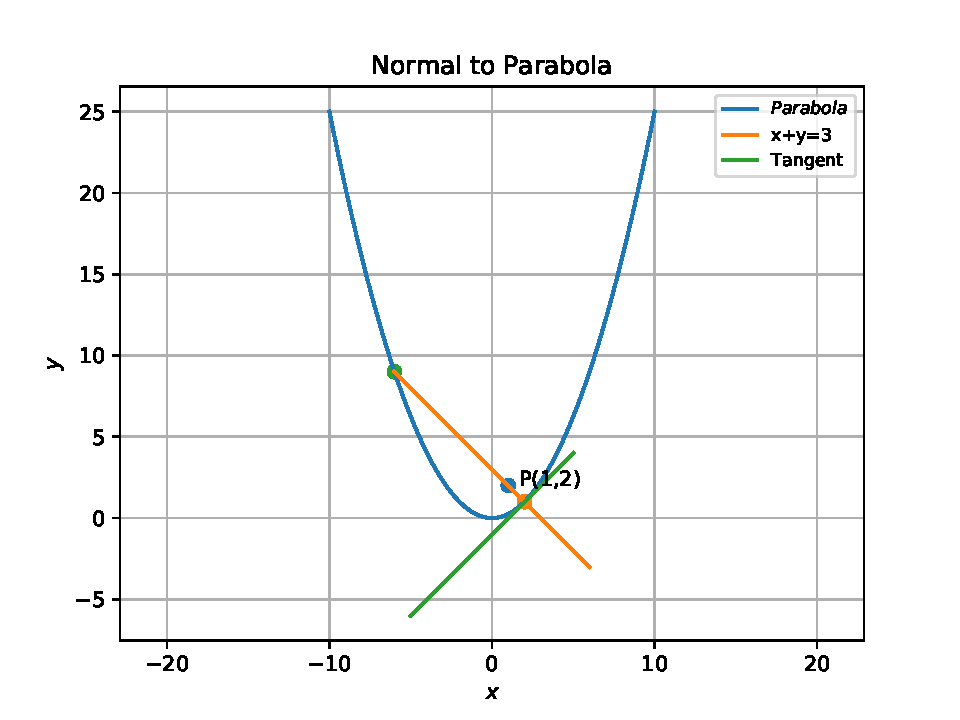
\includegraphics[width=\columnwidth]{figs/problem23.pdf}
	\end{center}
\caption{}
\label{fig:Fig1}
\end{figure}
\end{enumerate}
\end{document}
